\section{Linear layer}\label{sec:Linearappendix}
In the main paper, we defined the linear layer without the bias term for simplicity (\cref{def:linear_mainpaper}). In this section, we will redefine the linear layer with the bias term and present a comprehensive construction of the Linear Forward module.

\begin{definition}[Linear layer]\label{def:linear_appendix}
    For a weight $\mW\in\RR^{\aux{D} \times \aux{D}}$ and bias $\vb \in \RR^{ \aux{D} }$, a linear layer takes $\vx\in\RR^{\aux{D}}$ as input and outputs $\vy = \mW\vx + \vb$.
\end{definition}

In the discussions below, we consider a linear layer in the auxiliary model with parameters $\{\mW, \vb\}$ that takes in input sequence $\vx_1, \cdots, \vx_{\aux{T}}$ and outputs $\vy_1, \cdots, \vy_{\aux{T}}$, with $\vy_t = \mW \vx_t + \vb$ for each $t \le \aux{T}$. Since this involves a token-wise operation, we will present our constructed modules with a general token position $t$ and the prefix tokens $\{\vv_j\}.$ 


\paragraph{\simulator{} Linear Forward module} Continuing our discussion from \cref{sec:exposition_linear_forward}, we represent $S$ stacked rows of $\mW$ as a prefix embedding. In addition, we store the bias $\vb$ in the first prefix embedding ($\vv_1$).  

Using a set of $S'$ unique attention heads in a \simulator{} attention module (\cref{def:self-attn_construct}), we copy the bias $\vb$ to respective token embeddings and use a \simulator{} linear layer to add the biases to the final output.




\paragraph{Auxiliary's backpropagation through linear layer} For a linear layer as defined in \cref{def:linear_appendix}, the linear backpropagation layer takes in the loss gradient w.r.t. output ($\losspartial{\vy}$) and computes the loss gradient  w.r.t. input ($\losspartial{\vx}$).

\begin{definition}[Linear backpropagation ]\label{def:linear_backprop}
    For a weight $\mW\in\RR^{ \aux{D}  \times \aux{D} }$ , the linear backpropagation layer takes $\losspartial{ \vy } \in\RR^{ \aux{D} }$ as input and outputs $\losspartial{\vx} = \mW^{\top} \losspartial{\vy}$.
\end{definition}


\paragraph{\simulator{} Linear backpropagation module} 
%Correspondingly,
This module will aim to simulate the auxiliary's linear backpropagation.
The input embedding $\ve_t$ to this module will contain the gradient of the loss w.r.t. $\vy_t$, i.e. $\losspartial{  \vy_t }$. As given in \cref{def:linear_backprop}, this module will output the gradient of the loss w.r.t. $\vx_t$, given by $\losspartial{\vx_t} = \mW^{\top} \losspartial{\vy_t}.$ 

We first use the residual connection to copy the prefix embeddings $\{ \vv_j \}$ (i.e., the rows of $\mW$) from the forward propagation module.
%We first copy using the residual connection, the prefix embeddings $\{ \vv_j \}$ from the linear forward module, which contains the stacked rows of the matrix $\mW$. 
A straightforward construction would be to use the Linear Forward module but with the columns of $\mW$ stored in the prefix tokens, thereby simulating multiplication with $\mW^\top$.
However, such a construction requires applying attention to the prefix tokens, which increases the size of the construction substantially.
%To get the output, a simple strategy can be to use the linear forward module but with rows of $\mW^{\top}$ in the prefix tokens $\{\vv_j\},$ and bias set to $0$. However, this will involve additional attention modules (and hence additional training parameters) on the content of $\{\vv_j\}$ itself. 

We instead perform the operation more efficiently by splitting it across attention heads. In particular, once we view the operation as $\losspartial { \vx_t } = \sum_{i} \left(\losspartial { \vy_t } \right)_i \vw_i$, we can see that the attention score between the current token and the prefix token containing $\vw_i$ must be $\left(\losspartial {\vy_t } \right)_i$. Using value vectors as rows of $\mW$ returns the desired output.
Similar to the Linear Forward module, we shard the weights into $S'$ parts to parallelize across more attention heads. Please see \cref{fig:linear_back}.

%The more efficient strategy will be to view the required operation as $\losspartial { \vx_t } = \sum_{i} \left(\losspartial { \vy_t } \right)_i \vw_i$. 
%This can then be represented with  the attention heads, where for each attention head, the attention score between $\vv_j$, for any $j \le K$, and $\mathbf{e}_t$ is given by $\left(\losspartial {\vy_t } \right)_i$, with the value vector being $\vw_i$ for some $\vw_i$ stored in $\vv_j$. The linear projection layer will sum up the results of the attention heads. 

%each attention head represents the attention score between $\ve_t$ and $\vv_j$ that contains $\vw_i$ as $\left(\frac{\partial \loss}{\partial \vy_t}\right)_i$, with the value matrix using $\vw_i$.





\begin{figure}[t]
    \centering
    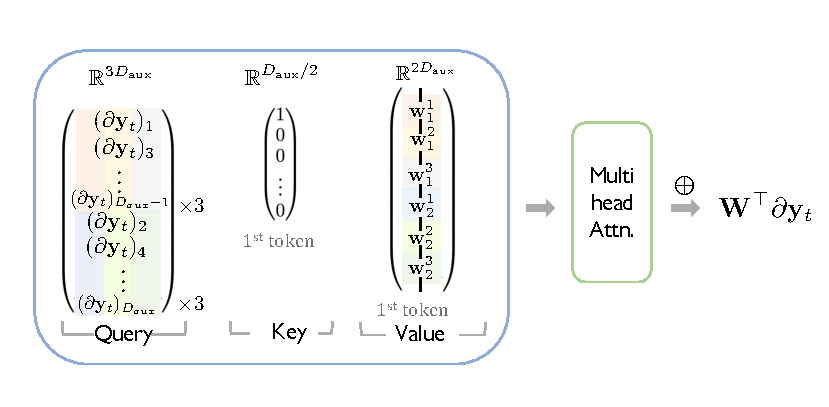
\includegraphics[width=0.7\textwidth]{figures/Linear_backward-cropped.pdf}
    \caption{\simulator{} simulates the backward pass of a linear layer as a $H$-head attention layer ($H=6$ pictured), with the gradient of the loss w.r.t. linear layer output ($\losspartial{\vy_t}$) as the query, the positional one-hot vector of prefix embeddings as the key, and the parameters of the auxiliary model stored in the prefix embeddings as the value. Similar to the Linear Forward module (\cref{fig:linear_forward}), we distribute the dot product computations across all attention heads by sharding the vectors into $S'$ ($S'=3$ here) parts. We omitted the identical transformation for query, and value matrices, and permutation-based transformation for key matrix for illustration purposes.}
    \label{fig:linear_back}
\end{figure}



\begin{figure}[t]
    \centering
    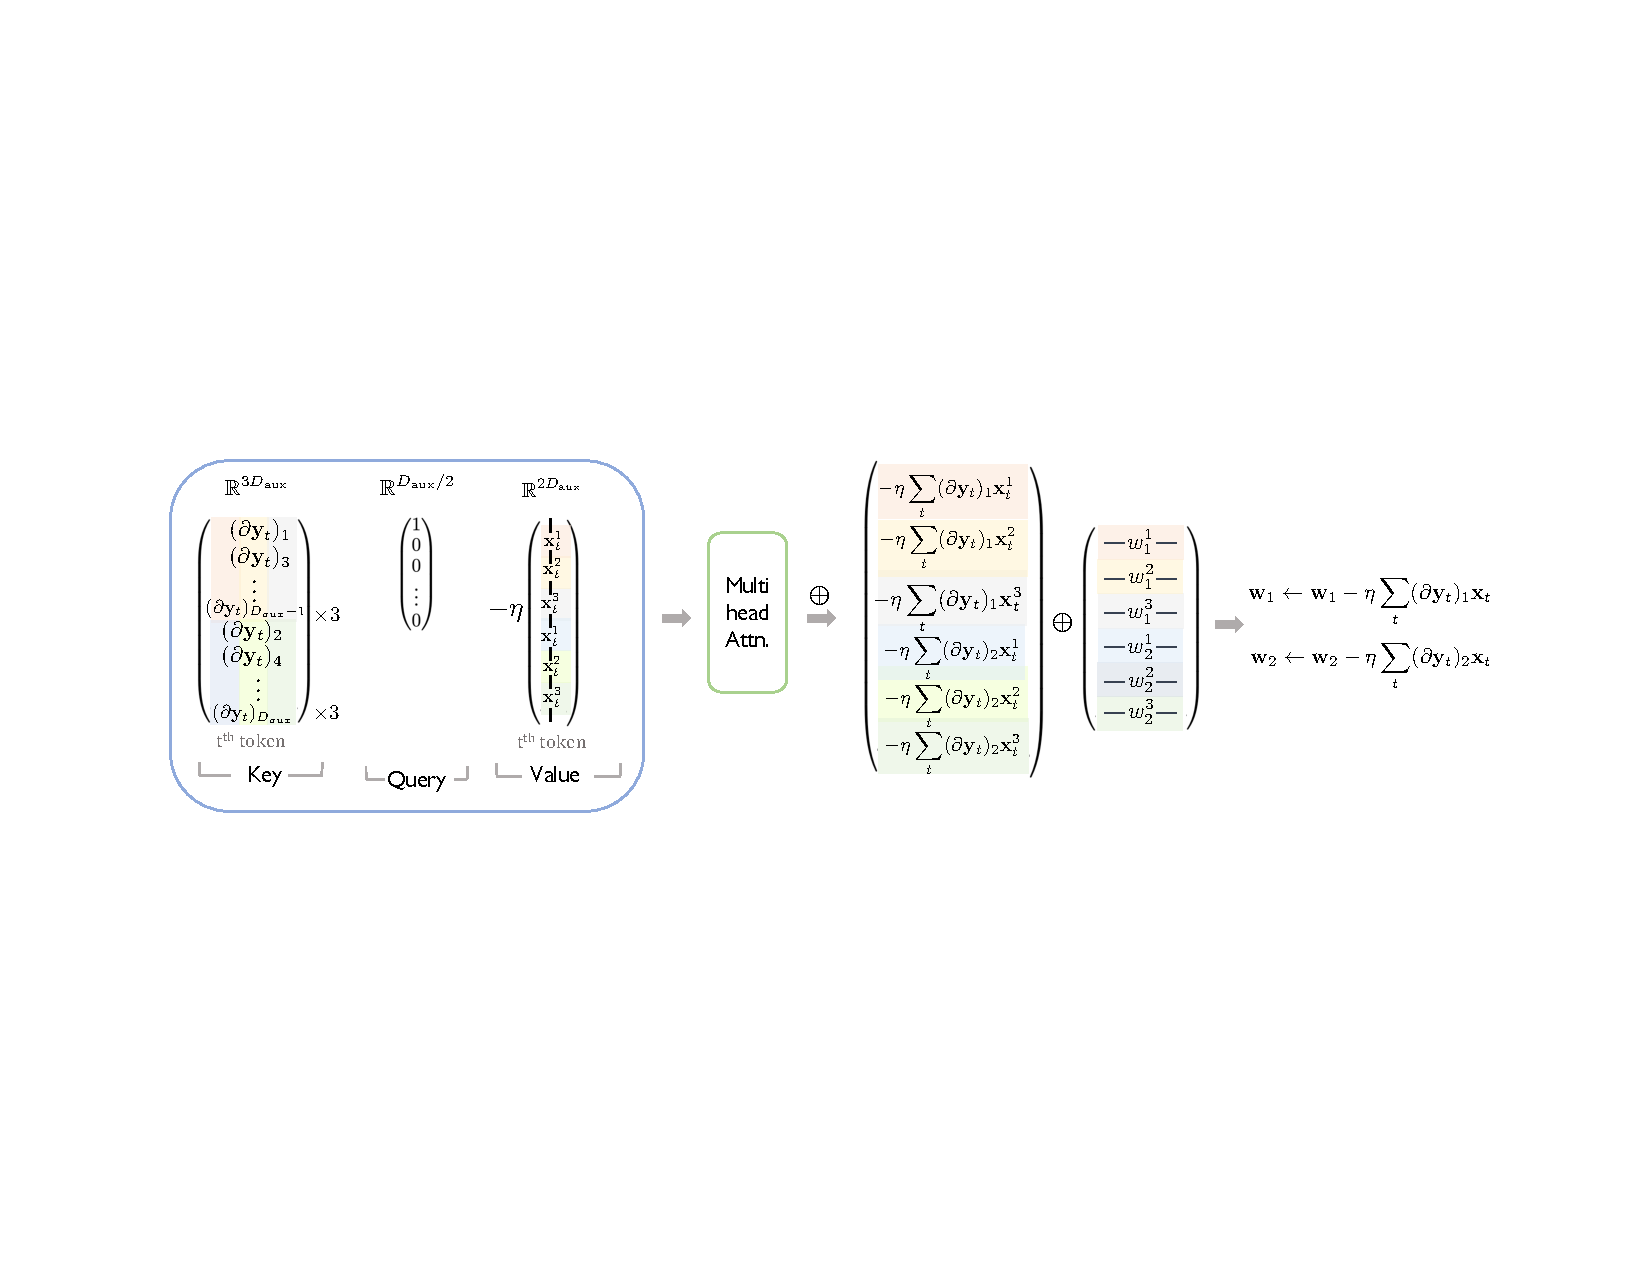
\includegraphics[width=\textwidth]{figures/Linear_descent_cropped.pdf}
    \caption{\simulator{} computes the parameter gradients for a linear layer as a $H$-head attention layer ($H=6$ pictured),  with  the gradient of the loss w.r.t. linear layer output ($\losspartial{\vy_t}$) as the query, the positional one-hot vector of prefix embeddings as the key, and  the input to the linear layer ($\vx_t$) as the value. The auxiliary model parameters in the prefix embeddings are then updated using a residual connection.
    Similar to the Linear Forward module (\cref{fig:linear_forward}), we distribute the dot product computations across all attention heads, by sharding the vectors into $S'$ ($S'=3$ here) parts. We omitted the identical transformation for query, and value matrices, and permutation-based transformation for key matrix for simplicity. }
    \label{fig:linear_descent}
\end{figure}






   



\paragraph{Auxiliary's linear descent update} Finally, the linear descent layer updates the weight and the bias parameters using a batch of inputs $\{\vx_t\}_{t \le {\aux{T}}}$ and the loss gradient w.r.t. the corresponding outputs $\{ \losspartial{\vy_t} \}_{t \le {\aux{T}}}$.

\begin{definition}[Linear descent]\label{def:linear_descent}
    For a weight $\mW\in\RR^{\aux{D}\times \aux{D}}$ and a bias $\vb \in \RR^{ \aux{D}}$, the linear descent layer takes in a batch of inputs $\{ \vx_t \in \RR^ \aux{D} \}_{t \le {\aux{T}}}$ and gradients $\{ \losspartial{\vy_t} \in \RR^ \aux{D} \}_{t \le {\aux{T}}}$ and updates the parameters as follows:
    \begin{align*}
        \mW \gets \mW - \eta \sum_{t \le {\aux{T}}} \losspartial{\vy_t} \vx_t^{\top}; \quad \quad
        \vb \gets \vb - \eta \sum_{t \le {\aux{T}}} \losspartial{\vy_t}.
    \end{align*}
\end{definition}

 

\iffalse
\begin{figure*}[t!]
    \centering
    \begin{subfigure}[t]{0.5\textwidth}
        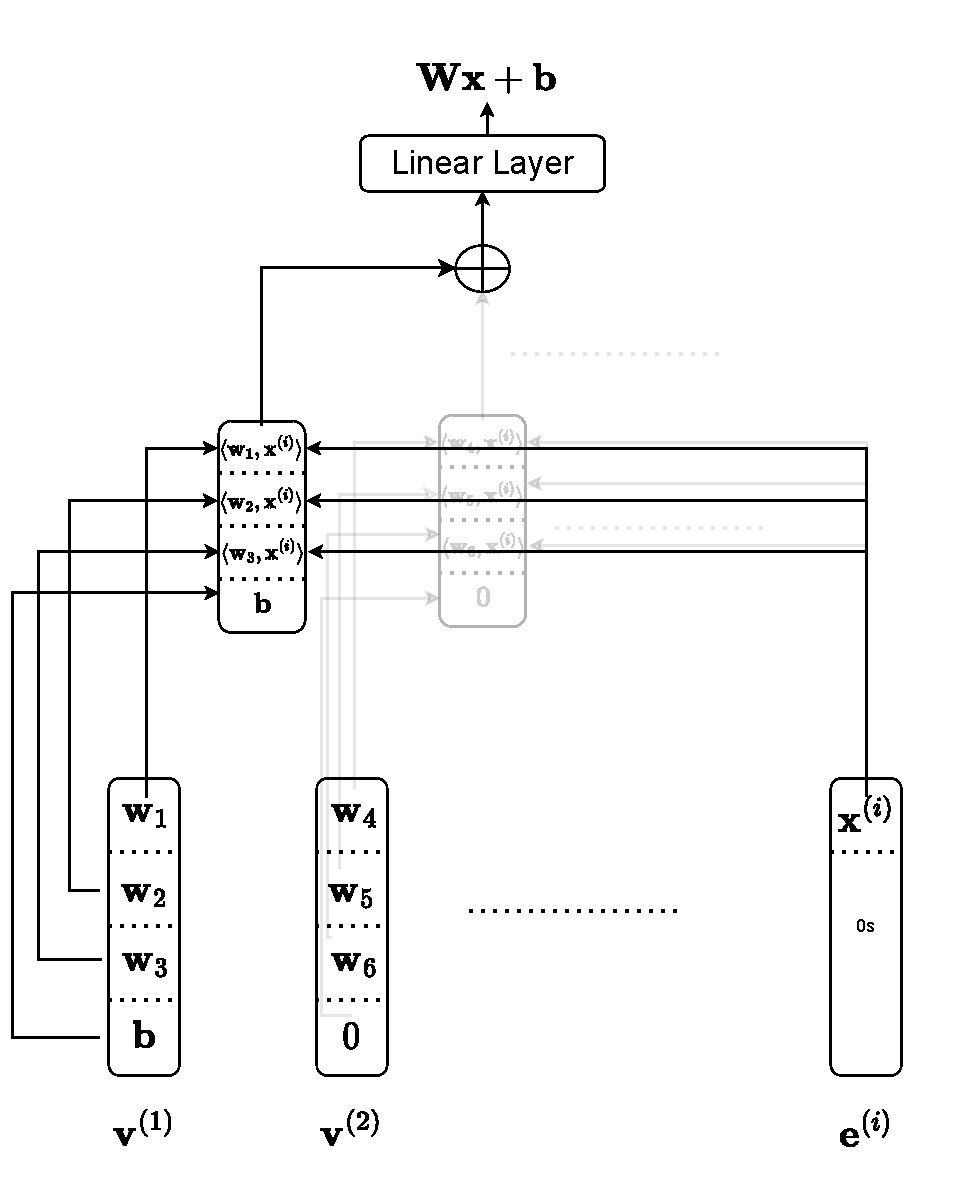
\includegraphics[width=\linewidth]{figures/ICL_linearforward.pdf}
        \caption{Forward}
    \end{subfigure}%
    ~ 
    \begin{subfigure}[t]{0.5\textwidth}
        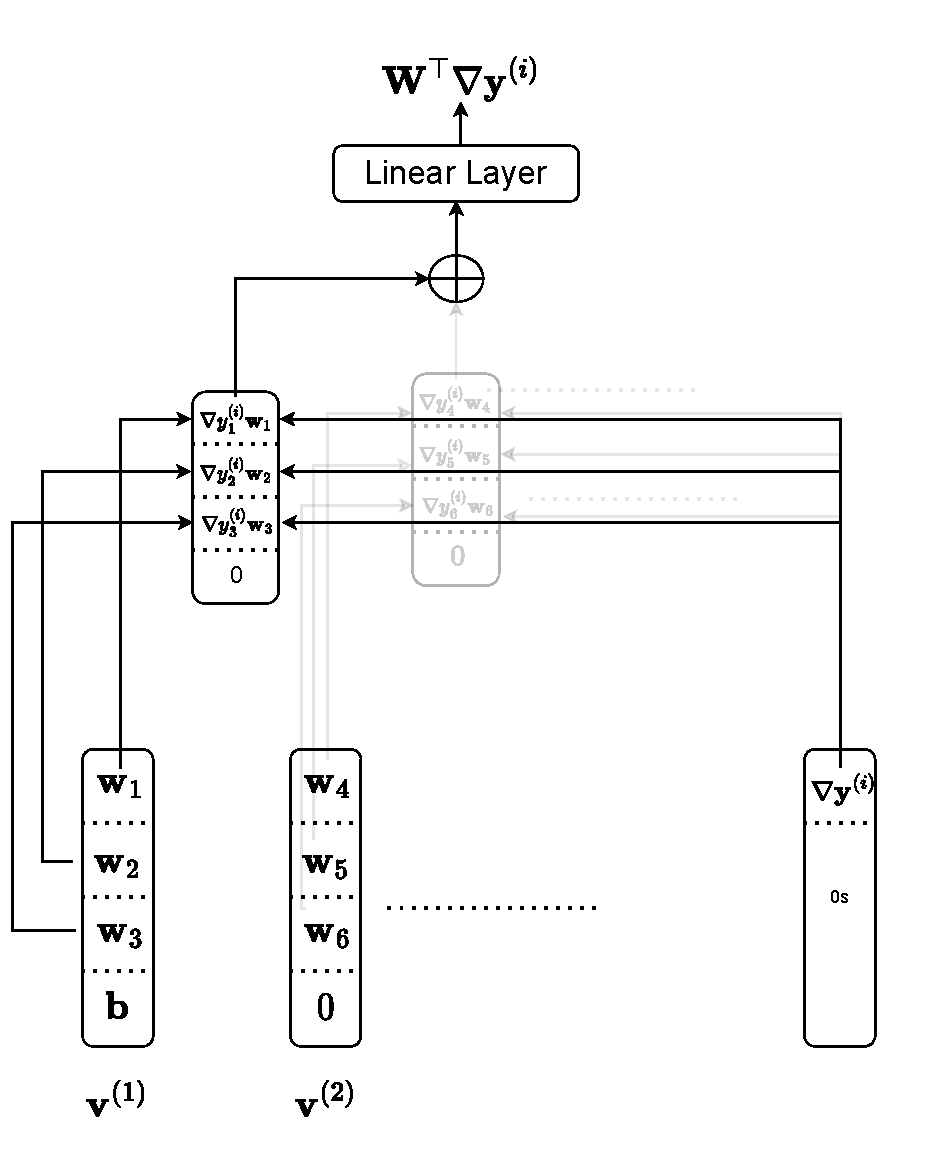
\includegraphics[width=\linewidth]{figures/ICL_linearback.pdf}
        \caption{Backward}
    \end{subfigure}
    \caption{Simulating forward and gradient backpropagation of a linear layer, shape of input is $batchsize \times (n+m) \times 4d$}
    \label{fig:general_structure_simulator}
\end{figure*}
\fi
\paragraph{\simulator{} Linear descent module} The input embedding $\ve_t$ to this module will contain the gradient of the loss w.r.t. $\vy_t$, i.e. $\losspartial{  \vy_t }$. 


As in the Linear backpropagation module, the prefix tokens $\{ \vv_j \}$ will contain the rows of  $\mW$ and $\vb$, which have been copied from the Linear forward module using residual connections. Since, in addition to the gradients, we also require the input to the linear layer, we will use residual connections to copy the input $\{ \vx_t \}$ to their respective embeddings $\{ \ve_t \},$ from the Linear Forward module. As given in \cref{def:linear_descent}, this module will update $\mW$ and $\vb$ using the gradient descent rule. 

%Since the update also requires $\vx_t$, we will use the residual connection to get $\vx_t$ from the Linear Forward module.

Focusing on $\vw_i$, the descent update is given by $\vw_i \gets \vw_i - \eta \sum_{t} \left( \losspartial { \vy_t } \right)_i \vx_t$. For the prefix token $\vv_j$ that contains $\vw_i$, the update term $- \eta \sum_{t} \left( \losspartial { \vy_t } \right)_i \vx_t$ can be expressed with an attention head that represents the attention between the prefix token $\vv_j$ and any token $\ve_t$ with score $\left( \losspartial { \vy_t } \right)_i$ and value $-\eta \vx_t$. The residual connection can then be used to update the weights $\vw_i$ in $\vv_j$. 

For the bias $\vb$, the descent update is give by $\vb \gets \vb - \eta \sum_{t} \losspartial { \vy_t } $. With $\vb$ present in $\vv_1$, we use one attention head to represent the attention score between prefix token $\vv_1$ and any token $\ve_t$ as $1$, with the value being $-\eta \losspartial{\vy_t}.$ The residual connection can then be used to update the weights $\vb$ in $\vv_1$. 


The above process can be further parallelized across multiple attention heads, by sharding each weight computation into $S'$ parts. Please see \cref{fig:linear_descent}.



\subsection{$\simu{H}$-split operation} \label{sec:H-split_operation_app}

We leverage local structure within the linear operations of \simulator{} to make the construction smaller. 
We build two $\simu{H}$-split operations to replace all the linear operations. We use $\simu{d}$ to denote $\simu{D}/\simu{H}$ in the following definitions. 
\begin{definition}[Split-wise $\simu{H}$-split Linear operation]
    For weight and bias parameters $\simuw{\mW} \in \RR^{\simu{H} \times \simu{d}  \times \simu{d}}, \simuw{\mB} \in \RR^{\simu{H} \times \simu{d}}$ , this layer takes in input $\ve \in \RR^{\simu{D}}$ and returns $\Tilde{\ve} = \attmerge( \Tilde{\mS}  + \simuw{\mB} )$, with $\Tilde{\mS} \in \RR^{\simu{H} \times \simu{d}} $ defined with rows $ \{ \simuw{\mW}_h \attsplit_{\simu{H}}(\ve)_h \}_ {h \le \simu{H} }$. 
\end{definition}

\begin{definition}[Dimension-wise $\simu{H}$-split Linear operation]
    For weight and bias parameters $\simuw{\mW} \in \RR^{\simu{d} \times \simu{H} \times \simu{H}}, \simuw{\mB} \in \RR^{\simu{d} \times \simu{H}}$ , this layer takes in input $\ve \in \RR^{\simu{D}}$, defines $\mS \in \RR^{\simu{d} \times \simu{H} }$ with columns $\{ \attsplit_{\simu{H}}(\ve)_h \}_{ h \le \simu{H} }$, and returns $\Tilde{\ve} = \attmerge( (\Tilde{\mS} + \simuw{\mB})^{\top} )$, where $\Tilde{\mS} \in \RR^{\simu{d} \times \simu{H}} $ is defined with rows $ \{ \simuw{\mW}_d \simuw{\vs}_d \}_ {d \le \simu{d} }$.
\end{definition}


We find that we can replace all the linear operations with a splitwise $\simu{H}$-split Linear operation followed by a dimensionwise $\simu{H}$-split Linear operation, and an additional splitwise $\simu{H}$-split Linear operation, if necessary. A linear operation on $\simu{D}$-dimensional space involves $\simu{D}^2$ parameters, while its replacement requires $\simu{D}^2/\simu{H} + 2\simu{D}\simu{H}$ parameters, effectively reducing the total number of necessary parameters by $\simu{H}$.



We motivate the $\simu{H}$-split linear operations with an example. We consider the Linear Forward module in \cref{fig:linear_forward} for simulating a linear operation with parameters $\mW \in \RR^{\aux{D} \times \aux{D}}$ and no biases. For simplicity of presentation, we assume $\aux{D}$ is divisible by $4$. We stack $2$ rows of weights per prefix embedding. We distribute the dot-product computation across the $\simu{H}=6$ attention heads, by sharding each weight into $3$ parts. Since we require to have enough space to store all the sharded computation from the linear attention heads, we require $\simu{D} = 3 \aux{D}$ (we get $3$ values for each of the $\aux{D}$ weights in $\mW$). 
For presentation, for a given vector $\vv \in \RR^{\aux{D}}$, we represent $\attsplit_{3} (\vv)_i$ by $\vv^i$ for all $1 \le i \le 3$.


Now, consider the final linear operation responsible for combining the output of the attention heads. The output, after the linear operation, should contain $\mW \vx_t$ in the first $\aux{D}$ coordinates.
At any position $t$, if we stack the output of the linear attention heads as rows of a matrix $\mS_t \in \RR^{ \simu{H} \times \simu{D} / \simu{H} }$ we get

\begin{align*}
    \mS_t  = \begin{bmatrix}
     \langle \vw_1^1, \vx_t^1 \rangle & \langle \vw_3^1, \vx_t^1 \rangle & \langle \vw_5^1, \vx_t^1 \rangle  & \cdots & \langle \vw_{\aux{D}-1}^1, \vx_t^1 \rangle  \\
     \langle \vw_1^2, \vx_t^2 \rangle & \langle \vw_3^2, \vx_t^2 \rangle & \langle \vw_5^2, \vx_t^2 \rangle  & \cdots & \langle \vw_{\aux{D}-1}^2, \vx_t^2 \rangle \\
     \langle \vw_1^3, \vx_t^3 \rangle & \langle \vw_3^3, \vx_t^3 \rangle & \langle \vw_5^3, \vx_t^3 \rangle  & \cdots & \langle \vw_{\aux{D}-1}^3, \vx_t^3 \rangle \\
     \langle \vw_2^1, \vx_t^1 \rangle & \langle \vw_4^1, \vx_t^1 \rangle & \langle \vw_6^1, \vx_t^1 \rangle  & \cdots & \langle \vw_{\aux{D}}^1, \vx_t^1 \rangle  \\
     \langle \vw_2^2, \vx_t^2 \rangle & \langle \vw_4^2, \vx_t^2 \rangle & \langle \vw_6^2, \vx_t^2 \rangle  & \cdots & \langle \vw_{\aux{D}}^2, \vx_t^2 \rangle\\
     \langle \vw_2^3, \vx_t^3 \rangle & \langle \vw_4^3, \vx_t^3 \rangle & \langle \vw_6^3, \vx_t^3 \rangle  & \cdots & \langle \vw_{\aux{D}}^3, \vx_t^3 \rangle
\end{bmatrix}
\end{align*}


Note that for each $j \le \aux{D}$, we have $ \langle \vw_j, \vx_t \rangle = \sum_{i=1}^{3}  \langle \vw_j^i, \vx_t^i \rangle$.  Thus, with a column-wise linear operation  on $\mS_t$, we can sum the relevant elements in each column to get
\begin{align*}
    &\mS^{col}_t  = \\& \begin{bmatrix}
     \langle \vw_1, \vx_t \rangle &  \langle \vw_3, \vx_t \rangle &   \cdots & \langle \vw_{ \aux{D}/2 - 1}, \vx_t \rangle  & 0 & 0  & \cdots & 0  \\
     \langle \vw_2, \vx_t \rangle &  \langle \vw_4, \vx_t \rangle &  \cdots & \langle \vw_{ \aux{D}/2 }, \vx_t \rangle  & 0 & 0  & \cdots & 0  \\
     0 &  0 & \cdots & 0  &  \langle \vw_{ \aux{D} / 2 + 1 }, \vx_t \rangle & \langle \vw_{ \aux{D} / 2 + 3 }, \vx_t \rangle  & \cdots & \langle \vw_{ \aux{D} - 1 }, \vx_t \rangle  \\
    0 &  0 &  \cdots & 0  &  \langle \vw_{ \aux{D} / 2 + 2 }, \vx_t \rangle & \langle \vw_{ \aux{D} / 2 + 4 }, \vx_t \rangle & \cdots & \langle \vw_{ \aux{D} }, \vx_t \rangle  \\
     0 &  0 &  \cdots & 0  &  0 &  0 & \cdots & 0   \\
     0 &  0 &  \cdots & 0  &  0 &  0 & \cdots & 0  
\end{bmatrix}
\end{align*}




A row-wise linear operation on $\mS^{col}_t$ can space out the non-zero elements in the matrix and give us
\begin{align*}
    &\mS^{row}_t  = \\& \begin{bmatrix}
     \langle \vw_1, \vx_t \rangle & 0 & \langle \vw_3, \vx_t \rangle & 0 &  \cdots & \langle \vw_{ \aux{D}/2 - 1}, \vx_t \rangle  & 0   \\
     0 & \langle \vw_2, \vx_t \rangle & 0 & \langle \vw_4, \vx_t \rangle &  \cdots & 0 & \langle \vw_{ \aux{D}/2 }, \vx_t \rangle   \\
     \langle \vw_{ \aux{D} / 2 +  1}, \vx_t \rangle & 0 & \langle \vw_{ \aux{D} / 2 +  3}, \vx_t \rangle & 0 &  \cdots & \langle \vw_{ \aux{D} - 1}, \vx_t \rangle  & 0   \\
    0 & \langle \vw_{ \aux{D} / 2 +  2}, \vx_t \rangle & 0 & \langle \vw_{ \aux{D} / 2 +  4}, \vx_t \rangle &  \cdots & 0 & \langle \vw_{ \aux{D} }, \vx_t \rangle   \\
     0 &  0 &  \cdots & 0  &    \cdots & 0 &  0   \\
     0 &  0 &  \cdots & 0  &    \cdots & 0 &  0  
\end{bmatrix}
\end{align*}




Finally, a column-wise linear operation on $\mS^{row}_t$ helps to get the non-zero elements in the correct order.
\begin{align*}
    &\Bar{\mS}^{col}_t  = \\&\begin{bmatrix}
     \langle \vw_1, \vx_t \rangle & \langle \vw_2, \vx_t \rangle & \langle \vw_3, \vx_t \rangle & \langle \vw_4, \vx_t \rangle  &  \cdots & \langle \vw_{\aux{D}/2-1}, \vx_t \rangle & \langle \vw_{\aux{D}/2}, \vx_t \rangle \\
     \langle \vw_{\aux{D}/2 + 1}, \vx_t \rangle & \langle \vw_{\aux{D}/2 + 2}, \vx_t \rangle & \langle \vw_{\aux{D}/2 + 3}, \vx_t \rangle & \langle \vw_{\aux{D}/2 + 4}, \vx_t \rangle  &  \cdots & \langle \vw_{\aux{D}-1}, \vx_t \rangle & \langle \vw_{\aux{D}}, \vx_t \rangle \\
     0 &  0 & 0 & 0   & \cdots & 0 & 0 \\
     \vdots & \vdots & \vdots & \vdots & \cdots & \vdots & \vdots \\
     0 &  0 & 0 & 0  & \cdots & 0 & 0
\end{bmatrix}
\end{align*}

The desired output is then given by $\attmerge( \{ \Bar{\vs}^{col}_{t, j} \} \}_{j=1}^{\aux{D}} )$, which contains $\mW \vx_t$ in the first $\aux{D}$ coordinates. The operations that convert $\mS_t$ to $\mS_t^{col}$ and $\mS_t^{row}$ to $\Bar{\mS}_t^{row}$ represents a split-wise $6$-split linear operation, while the operation that converts $\mS^{col}_t$ to $\mS_t^{row}$ represents a dimension-wise $6$-split linear operation. A naive linear operation on the output of the attention heads would require $\simu{D}^2$ parameters, while its replacement requires $\simu{D}^2/6$ parameters to represent a dimension-wise $6$-split linear operation, and an additional $12 \simu{D}$ parameters to represent the split-wise $6$-split linear operations.



%We follow a similar approach as the backpropagation module, since the gradient descent update for $\vw_i$ can be represented as $\vw_i \gets \vw_i - \eta \sum_{t} \left( \losspartial { \vy_t } \right)_i \vx_t$. 

%This can then be represented with a single attention head, which computes the attention score between $\vv_j$ containing $\vw_i$, and $\mathbf{e}_t$ by $\left(\losspartial { \vy_t }\right)_i$, with the value vector being $-\eta \vx_t$. The residual connection will be used to update the weights $\vw_i$ in $\vv_j$. 


